%!TEX root = ../thesis.tex
% створюємо розділ
\chapter{Застосування глибинного навчання у моделюванні розвитку простих організмів}
\label{chap:theory}

Щось на мові вступу.

\hide{
До другого розділу також краще написати малесенький вступ. Зокрема, це 
збільшує загальний об'єм роботи та покращує її читабельність.
}

%%%%%%%%%%%%%%%%%%%%%%%%%%%%%%%%%%%%%%%%%%%%%%%%%%%%%%%%%%%%%%%%%%%%%%%%%%%%%%%
\section{Нейронні мережі}





%%%%%%%%%%%%%%%%%%%%%%%%%%%%%%%%%%%%%%%%%%%%%%%%%%%%%%%%%%%%%%%%%%%%%%%%%%%%%%%
\section{Навчання нейронної мережі за допомогою генетичних алгоритмів}



%%%%%%%%%%%%%%%%%%%%%%%%%%%%%%%%%%%%%%%%%%%%%%%%%%%%%%%%%%%%%%%%%%%%%%%%%%%%%%%
\section{Процес моделювання розвитку простих організмів}



%%%%%%%%%%%%%%%%%%%%%%%%%%%%%%%%%%%%%%%%%%%%%%%%%%%%%%%%%%%%%%%%%%%%%%%%%%%%%%%
\hide{
У другому розділі необхідно наводити розв'язання поставленої перед вами 
задачі у теоретичному або аналітичному сенсі (хоча, звісно, все залежить 
від того, яка саме задача перед вами поставлена).

Для подання матеріалів можна використовувати таблиці (наприклад, 
Таблицю \ref{tab_weight}). Розмір шрифту у таблиці може бути меншим за 14~pt (наприклад, 12~pt, або навіть 10~pt, якщо так таблиця виглядає зрозуміліше та компактніше).

    \begin{table}[ht]
    \setfontsize{14pt}
    \caption{Розрахунок якоїсь фантастичної дичини у декілька кроків}
    \label{tab_weight}
    \centering
        \begin{tabular}{|c|c|c|c|c|c|c|c|c|}
        \hline \multirow{2}{*}{Параметр $x_i$} & \multicolumn{4}{c|}{Параметр $x_j$} & 
            \multicolumn{2}{c|}{Перший крок} & \multicolumn{2}{c|}{Другий крок} \\
        \cline{2-9} & $X_1$ & $X_2$ & $X_3$ & $X_4$ & $w_i$ & 
            ${K_\text{в}}_i$ & $w_i$ & ${K_\text{в}}_i$ \\
        \hline $X_1$ & 1 & 1 & 1.5 & 1.5 & 5 & 0.31 & 19 & 0.32 \\
        \hline $X_2$ & 1 & 1 & 1.5 & 1.5 & 5 & 0.31 & 19 & 0.32 \\
        \hline $X_3$ & 0.5 & 0.5 & 1 & 0.5 & 2.5 & 0.16 & 9.25 & 0.16 \\
        \hline $X_4$ & 0.5 & 0.5 & 1.5 & 1 & 3.5 & 0.22 & 12.25 & 0.20 \\
        \hline \multicolumn{5}{|c|}{Разом:} & 16 & 1 & 59.5 & 1 \\
        \hline
        \end{tabular}
    \end{table}

Бажано, щоб кожен пункт завдань, окреслених у вступі, відповідав певному 
розділу або підрозділу у дипломній роботі.
}


\hide{

% \section{(Якийсь наступний підрозділ з дуже-дуже довгою назвою, загальна кількість слів в якій, однак, не повинна перевищувати 12 слів)}

Для подання матеріалів також дуже зручними є рисунки (наприклад, рисунки 
\ref{fig_sudak} або \ref{fig_pacman}).
}


\hide{
\begin{figure}[ht]
\centering
    \begin{subfigure}[b]{0.5\textwidth}    
        
\includegraphics[scale=0.3]{Images/Sudak.png}
        \caption{}
        % обратите внимание на знак % после \end{subfigure} и 
        % отсутствие пустых строк и разделителей после \end{subfigure}
        % -- это сливает в одну строку подфигуры
    \end{subfigure}%
    \begin{subfigure}[b]{0.5\textwidth}
        
\includegraphics[scale=0.3]{Images/Tudak.png}
        \caption{}
    \end{subfigure}
 
    \caption{Різні види риб: (a) судак, (б) тудак.}
    \label{fig_sudak}
\end{figure}

\begin{figure}[ht]
        \centering
        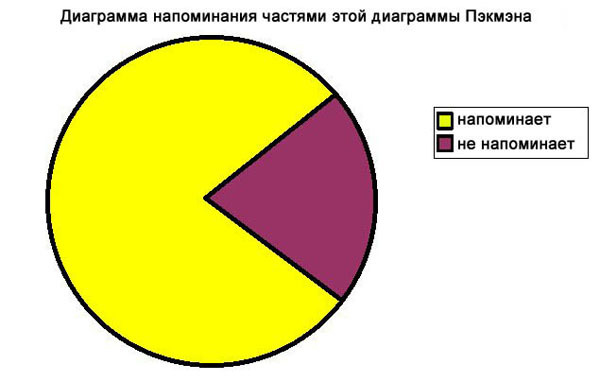
\includegraphics[scale=0.5]{Images/Pacman.jpg}
        \caption{Частка кругових діаграм, які схожі на Пекмена}
        \label{fig_pacman}
\end{figure}
}


%%%%%%%%%%%%%%%%%%%%%%%%%%%%%%%%%%%%%%%%%%%%%%%%%%%%%%%%%%%%%%%%%%%%%%%%%%%%%%%

\chapconclude{\ref{chap:theory}}

Наприкінці розділу знову наводяться коротенькі підсумки.
